\documentclass[]{article}
\usepackage{amsmath}\usepackage{amsfonts}
\usepackage[margin=1in,footskip=0.25in]{geometry}
\usepackage{mathtools}
\usepackage{hyperref}
\hypersetup{
    colorlinks=true,
    linkcolor=blue,
    filecolor=magenta,
    urlcolor=cyan,
}
\usepackage[final]{graphicx}
\usepackage{listings}
\usepackage{courier}
\lstset{basicstyle=\footnotesize\ttfamily,breaklines=true}

% \usepackage{wrapfig}
\graphicspath{{.}}

\begin{document}
\begin{center}
    Name: Honda Li \quad Class: CSE 546 SPRING 2021\quad HW3A
\end{center}

\section*{A1: Conceptual Questions}
    \subsection*{A.1.a}
        Decraese $\sigma$. This makes the function $\exp\left(
            - \frac{\Vert u - v\Vert_2^2}{2\sigma^2} 
        \right)$ thinner, make the inner product between different points more distinct. 
    \subsection*{A.1.b}
        True. It's an non-convex objective function, assuming thta deep means more than one hidden layer of course and assuming that activation function is not linear. 
    \subsection*{A.1.c}
        Yes it is. This ties to the fact that the Loss function of the Neural net is not convex, and if we start near all zeros, that means the first few iterations of the Gradient descent will aways get the same gradient, hugely limiting weight configuration of the model.
    \subsection*{A.1.d}
        Flase, the what gives non linear decision boundary is the number of layers and the number of neurons in the layers, both ReLU and the Sigmoid functions is using linear decision boundary under the hood, \textbf{it's a lot of linear decision bounary combined together}. 
    \subsection*{A.1.e}
        False if we use dynamic programming when doing backprop, else it's True. 
        \\
        Backward pass requires it goes for the Loss Layer to each layer to compute the gradient, but when computing the gradient of a $w_{i, j}^{(k)}$ at the $k$ th layer, because we already did a forward pass, therefore all the previous value for $w_{i, j}^{(k)}$ (where $0\le k< N$) were in the memory, so are the $a^{(k)}$ ($1\le k N$) . When doing backprop, we would need all the weight matrix at layer $N, N-1, N-2 \cdots k - 2$, and then we will need one row of $w_{i, j}^{(k - 1)}$, and $a_i^{(k-1)}$ to compute it. But all the previous big matrices are stored in the memory, and when we did the backward on $k-1$ layer therefore we already have all partials for $k-1, k - 2... N$. So using dynamic programming, we can save a lot of complexity, making it the same as forward pass. 

\section*{A.2: Kernels And Bootstrap}
    Give na vector whose $n$ th components paramterized by $n$ is given by: 
    $$
        \frac{1}{\sqrt{n!}}\exp \left(
            \frac{-x^2}{2}
        \right)x^n
    $$
    where $x$ is one dimensional, and the feature mapping function $\phi(x)$ is an infinite dimensional function. 
    \\
    Then: 
    \begin{align*}\tag{A.2.1}\label{eqn:A.2.1}
        \langle \phi(x), \phi(y)\rangle &= 
        \sum_{n = 1}^{\infty}
            \phi_n(x)\phi_n{y}
        \\
        &= 
        \sum_{n = 1}^{\infty}
            \frac{1}{\sqrt{n!}} 
            \exp \left(
                -\frac{x^2}{2}
            \right)x^n
            \frac{1}{\sqrt{n!}} 
            \exp \left(
                -\frac{y^2}{2}
            \right)y^n
        \\
        &= 
        \sum_{n = 1}^{\infty}
            \frac{(xy)^n}{n!}\exp\left(
                -\frac{x^2 + y^2}{2}
            \right)
        \\
        &= 
        \exp\left(
                -\frac{x^2 + y^2}{2}
            \right)
        \sum_{n = 1}^{\infty}
        \frac{(xy)^n}{n!}
        \\
        &= 
        \exp\left(
            - \frac{x^ 2 + y^ 2}{2}
        \right)
        \exp\left(
            xy
        \right)
        \\
        &= 
        \exp\left(
            - \frac{x^ 2 + y^ 2}{2} + \frac{2xy}{2} 
        \right)
        \\
        &= 
        \exp\left(
            \frac{-(x - y)^2}{2}
        \right)
    \end{align*}

    And this is the RBF kernel for a scalar, in the 1d case. 
    
\section*{A.3: Kernel Ridge Regression}
    For problem A.3, this is the core routine I used for the whole problem, filename: ``kernel\_ridge\_regression''
    \begin{lstlisting}[language=python]
### This is a script for CSE 546 SPRING 2021, HW3, A.3
### Implementing the kernel ridge regression and visualize some stuff.
### Author: Hongda Li

import numpy as np
from scipy import linalg
import matplotlib.pyplot as plt

linspace = np.linspace
randn = np.random.randn
pinvh = linalg.pinvh
inv = linalg.inv
eye = np.eye
mean = np.mean
std = np.std

class KernelRidge:

    def __init__(this, regularizer_lambda, kernelfunc: callable):
        """

        :param regularizer_lambda:
        :param kernelfunc:
            Takes in the WHOLE traning matrix and compute the kenrnel matrix K.

        """
        this.Lambda = regularizer_lambda
        this.KernelMatrix = None
        this.X = None
        this.Kernel = kernelfunc
        this.Alpha = None
        this.Bias = None

    @property
    def w(this):
        if this.X is None: return None
        return this.X.T@this.Alpha

    def fit(this, X, y):
        """

        :param x:
        :param y:
        :return:
        """
        assert type(X) is np.ndarray and type(y) is np.ndarray, "X, y, must be numpy array"
        assert X.ndim == 2 and y.ndim <= 2
        Warn = "X, y dimension problem"
        if y.ndim == 2:
            assert y.shape[0] == X.shape[0], Warn
            assert y.shape[1] == 1, Warn
        else:
            assert y.shape[0] == X.shape[0], Warn
            y = y[:, np.newaxis]
        assert X.shape[0] >= 1, "Need more than just one sample. "
        # Standardized.
        this.X = X
        n, d = X.shape
        Lambda = this.Lambda
        K = this.Kernel(this.X, this.X)
        assert K.ndim == 2 and K.shape[0] == K.shape[1] and K.shape[0] == n, \
            "your kernel function implemention is wrong, kernel matrix is having the wrong shape"
        assert np.all(np.abs(K-K.T) < 1e-5), "kernel matrix is not symmetric."
        this.KernelMatrix = K
        # get the bias

        # get the alpha.
        this.Alpha = pinvh(K + Lambda*eye(n))@y


    def predict(this, Xtest):
        assert this.X is not None, "Can't predict when not trained yet. "
        Xtrain = this.X
        return this.Kernel(Xtest, Xtrain)@this.Alpha



def main():
    def SimpleTest():
        N = 100
        w, b = 1, 0
        x = linspace(-1, 1, N)
        eps = randn(N)*0.1
        y = w*x + b + eps
        X = x[:, np.newaxis]
        def KernelFunc(X, Y):
            return X@Y.T
        Model = KernelRidge(regularizer_lambda=0.01, kernelfunc=KernelFunc)
        Model.fit(X, y)
        Yhat = Model.predict(X)
        plt.plot(x, y)
        plt.plot(x, Yhat)
        plt.show()
    SimpleTest()


if __name__ == "__main__":
    main()
    \end{lstlisting}
    \subsection*{A.3.a}
        To implement, we will need to take care of the process of solving for the best parameter $\alpha$, and we will also need to careful about the offset. So what we are going to train is on the zero mean data, and then the prediction made from the model will have to add back the offset from the training set of course. 
        \\
        Here is basically what we had from the sections: 
        \begin{align*}\tag{A.3.a}\label{eqn:A.3.a}
            \frac{1}{2}\nabla_x[\Vert K\alpha - y\Vert_2^2 + \lambda \alpha^T K \alpha] &= 0
            \\
            \implies K^T(K\alpha - y) + \lambda K\alpha &= 0
            \\
            K(K\alpha - y) + \lambda K\alpha &= 0
            \\
            KK\alpha - Ky + \lambda K\alpha &= 0
            \\
            KK\alpha + \lambda K\alpha &= Ky
            \\
            K \alpha + \lambda \alpha &= y
            \\
            \alpha &= (K + \lambda I)^{-1}y
        \end{align*}
        Where, $K$ and $y$ are from the training set. And in this case, the predictor can be computed via: $K_{\text{test}, \text{train}}\alpha$ where the $K_{\text{test}, \text{train}}$ is computed via: 
        $$
            K_{i, j} = \langle \phi(X_{\text{test}}[i, :]), 
                                \phi(X_{\text{train}}[:, j]) 
            \rangle
        $$
        
        To implement the method, I used the following tricks: 
        \begin{enumerate}
            \item[1.] All the questions from a, b, c, d, e, are running on a fixed sample. When I do the black box optimization, and grid search for hyper parameter, I want to make the whole algorithm deterministic, given a certain sample set. 
            \item[2.] I used a black box optimization to improve the grid search algorithm, The algorithm is SHGO, Simplicial Homology Global Optimization. It's used as a bounded non-convex optimization algorithm as a subroutine for the grid search algorithm.  
            \item[3.] I used the footnote information to narrow down the serach for the parameters of the Guassian model.  
        \end{enumerate}
        \textbf{Note}: That hyperparameter search algorithm I wrote runs forever. 
        \textbf{Note}: For 30 samples, there are a lot of variance on the models, and here is one of the hyper parameter identified by my algorithm: 
        \begin{enumerate}
            \item [1.] For poly kernel: $d = 28.06$, $\lambda = 0.0013477$. 
            \item [2.] For the KBF kernel: $\gamma = 31.5238$, $\lambda = 0.001119$. 
        \end{enumerate}

    \subsection*{A.3.b}
        This is the plot I had for the particular identified hyper parameters: 
        \begin{center}
            \includegraphics*[width=12cm]{A3b-poly.png}
        \end{center}
        \begin{center}
            \includegraphics*[width=12cm]{A3b-gauss.png}
        \end{center}
        
    \subsection*{A.3.c}
        For building the boopstrap, this is something about the implementation that I think it's worth noting: 
        \begin{enumerate}
            \item [1.] I am still using the same set of samples that produces the hyperparameters. 
            \item [2.] Because of huge variance for the poly model at the boundary of the data set, I have to scale the graph so that we can see what is happening, instead of zooming out like crazy. 
        \end{enumerate}
        Here is the graph for both the model: 
        \begin{center}
            \includegraphics*[width=12cm]{Poly-boopstraped.png}
        \end{center}
        \begin{center}
            \includegraphics*[width=12cm]{gaussian-boopstraped.png}
        \end{center}
        And there are a lot of variance. Very dependent on the sample too. 
    \subsection*{A.3.d}
        This is the repeated experiement with a sample size of $300$ and a $10$ Fold cross validation: 
        \begin{center}
            
\includegraphics[width=10cm]{hypertune300/A3b-poly.png}
            
\includegraphics[width=10cm]{hypertune300/A3b-gauss.png}
        \end{center}
        And this is the confident bands I placed on these models: 
        \begin{center}
            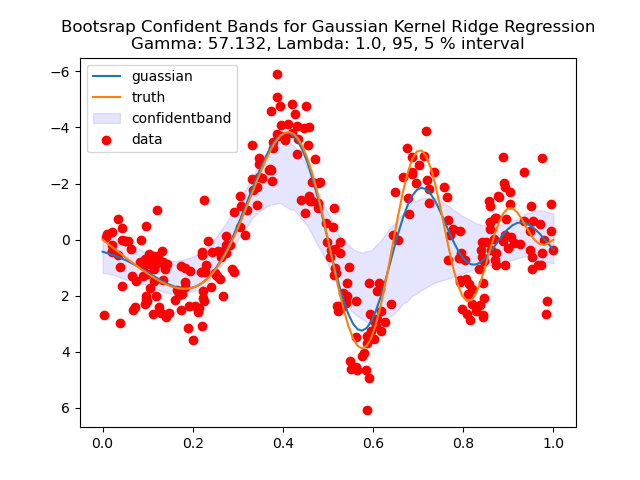
\includegraphics[width=10cm]{hypertune300/gaussian-boopstraped.png}
            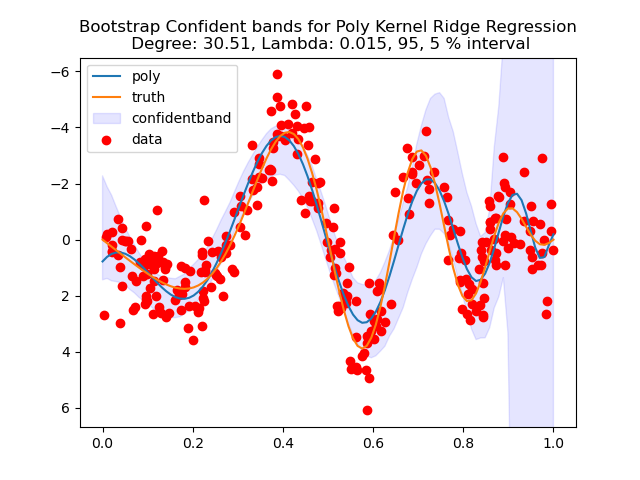
\includegraphics[width=10cm]{hypertune300/Poly-boopstraped.png}
        \end{center}
    \subsection*{A.3.e}
        And for those 2 particular models I got on the previous part for the problem, I ran the algorithm and bootstrapped the difference, and it turns out that this is the confident interval for the L2 norm error difference: 
        $$(0.08477231069630578, 0.15565650293476457)$$
        And it's larger than zero for both upper and lower bound. Therefore, the conclusion is that, the polynomial model is having a larger error. 
    \subsection*{A.3.Code}
        This is the main driver code I used for all the questions, it's quiet complicated so I have put it in the end of the section. 
        \\
        File name: ``A3.py''
        \begin{lstlisting}[language=python]
### This is the script that produce plots and data for A3
### This is for CSE 546 SPRING 2021, HW3.
### Author: Hongda Alto Li
### Requries: kernel_ridge_regression.py


import numpy as np
cos, sin, pi = np.cos, np.sin, np.pi
rand, randn, randint = np.random.rand, np.random.randn, np.random.randint
norm = np.linalg.norm
zeros = np.zeros
mean = np.mean
sum = np.sum
min = np.min
max = np.max
linspace = np.linspace
logspace = np.logspace
percentile = np.percentile
var = np.var
from kernel_ridge_regression import KernelRidge
from sklearn.metrics.pairwise import rbf_kernel, polynomial_kernel
from sklearn.model_selection import KFold
import matplotlib.pyplot as plt
from scipy.optimize import minimize, shgo
from scipy.optimize import Bounds

### Some constant for the whole script:




def RBFKernel(X, Y, gamma):
    """
        Use this kernel to take the inner products between the columns of X, Y
    :param x:
    :return:
    """

    return rbf_kernel(X, Y, gamma=gamma)


def MyPolyKernel(X, Y, d):
    """
        Use this kernel to take the inner product between the columns of the X, Y
        matrix.
    :param x:
    :return:
    """
    if Y is None: X = Y
    return polynomial_kernel(X, Y, gamma=1, degree=d)


def CrossValErrorEstimate(X, y, regualarizer, kernelfunc, split=None,param_norm=False):
    Errors = []
    AlphaNorm = []
    if split is None:
        split = X.shape[0]
    kf = KFold(n_splits=split, shuffle=False) # Make it deterministic given the same training sample.

    for TrainIdx, TestIdx in kf.split(X):
        Model = KernelRidge(regularizer_lambda=regualarizer, kernelfunc=kernelfunc)
        Model.fit(X[TrainIdx], y[TrainIdx])
        yhat = Model.predict(X[TestIdx]).reshape(-1)
        Error = (sum(yhat - y[TestIdx])**2)/len(TestIdx)
        Errors.append(Error)
        AlphaNorm.append(norm(Model.w, np.inf))
    if param_norm:
        return mean(Errors), min(AlphaNorm)
    return mean(Errors)


def GenerateXY(n):
    f = lambda x: 4 * sin(pi * x) * cos(6 * pi * x ** 2)
    x = rand(n)
    x.sort()
    y = f(x) + randn(n)
    return x[:, np.newaxis], y


def main(n=30, KfoldSplit=30):
    X, y = GenerateXY(n)   #  THIS IS SHARED! FOR ALL
    f = lambda x: 4 * sin(pi * x) * cos(6 * pi * x ** 2)
    def PolyKernelHypertune():
        def GetError(deg, l):
            Kernefun = lambda x, y: MyPolyKernel(x, y, deg)
            Error = CrossValErrorEstimate(X,
                                          y,
                                          regualarizer=l,
                                          kernelfunc=Kernefun,
                                          split=KfoldSplit)
            return Error
        BestError = float("inf")
        Best = None
        for Deg in np.linspace(7, 31):
            Result = shgo(lambda x: GetError(Deg, x),
                bounds=[(0, 0.05)],
                n=100,
                sampling_method="simplicial",
                options={"f_tol": 1e-8}
                          )
            if Result.fun < BestError:
                print(f"Poly Kernel Best error update for deg: {Deg}, Lambda: {Result.x}, Error: {Result.fun}")
                BestError = Result.fun
                Best = (Deg, Result.x[0])
            else:
                print(f"failed at: deg: {Deg}, Lambda: {Result.x[0]}, Error: {Result.fun}")

        # Result = shgo(lambda x: GetError(x, 0),
        #      bounds=[(1, 100)],
        #      n=200, sampling_method="simplicial",
        #               options={"f_tol": 1e-8, "disp": True})
        # print(f"SHGO Optimization Results: {Result}")
        return Best

    def GaussianKernelHypertune():
        # Grid search, Fix the training sample
        # X, y = GenerateXY()
        Xs = X.reshape(-1)
        Distance = []
        for II in range(Xs.size):
            for JJ in range(II + 1, Xs.size):
                Distance.append(1/(norm(Xs[II] - Xs[JJ])**2))
        GammaLower, GammaHigher = \
            percentile(Distance, 25), percentile(Distance, 75)
        print(f"Hypertune Gamma kernel search range: {GammaLower, GammaHigher}")
        def GetError(gamma, l):
            l, gamma = abs(l), abs(gamma)
            Kernelfun = lambda x, y: RBFKernel(x,y, gamma=gamma)
            Error = CrossValErrorEstimate(X,
                                          y,
                                          regualarizer=l,
                                          kernelfunc=Kernelfun,
                                          split=KfoldSplit
                                          )
            return Error
        # GRID SEARCH INITIAL GUESS
        Result = shgo(lambda x: GetError(x[0], x[1]),
                      bounds=[(GammaLower, GammaHigher), (0, 1)],
                      n=500, sampling_method='sobol',
                      options={"f_tol": 1e-4, "disp": True})
        print("Optimization results: ")
        print(Result)
        print(f"Guassian Bestparams: {Result.x}")
        return Result.x
    # ============ Hyper Param! ================================================
    GaussianBest = [20, 0.058]
    PolyBest = [19, 0.05]

    GaussianBest = GaussianKernelHypertune()
    PolyBest = PolyKernelHypertune()

    print(f"guassian kernel best is: [gamma, lambda] {GaussianBest}")
    print(f"Poly kernel best is: [deg, lambda] {PolyBest}")

    def DrawPolyModel():
        x = linspace(0, 1, 1000)
        Model = KernelRidge(regularizer_lambda=PolyBest[1],
                            kernelfunc=
                            lambda X, Y: MyPolyKernel(X, Y, PolyBest[0]))
        Model.fit(X, y)
        plt.ylim([max(y)*1.1, min(y)*1.1])
        plt.plot(x, Model.predict(x[:, np.newaxis]).reshape(-1))
        plt.plot(x, f(x))
        plt.scatter(X.reshape(-1), y, c="red")
        plt.title(f"poly kernel ridge regression\n "
                  f"degree: {PolyBest[0]}, lambda: {PolyBest[1]}")
        plt.xlabel("x")
        plt.ylabel("y")
        plt.legend(["Poly", "Truth", "Data Points"])
        plt.savefig("A3b-poly.png")
        plt.show()
        return Model

    BestPolyModel = DrawPolyModel()

    def DrawGuassianModel():
        x = linspace(0, 1, 1000)
        Model = KernelRidge(regularizer_lambda=GaussianBest[1],
                            kernelfunc=
                            lambda X, Y: RBFKernel(X, Y, GaussianBest[0])
                            )
        Model.fit(X, y)
        plt.ylim([min(y)*1.1, max(y)*1.1])
        plt.plot(x, Model.predict(x[:, np.newaxis]).reshape(-1))
        plt.plot(x, f(x))
        plt.scatter(X.reshape(-1), y, c="red")
        plt.title(f"guassian kernel ridge regression\n "
                  f"gamma: {GaussianBest[0]}, lambda: {GaussianBest[1]}")
        plt.xlabel("x")
        plt.ylabel("y")
        plt.legend(["Gaussian", "Truth", "Data Points"])
        plt.savefig("A3b-gauss.png")
        plt.show()
        return Model

    BestGaussianModel = DrawGuassianModel()

    # --------------------------------------------------------------------------
    # Boopstrap and estimating the confident interval.

    def BoopStraping(Kernelfunc, Lambda, x):
        # Given the kernel func, produce the confidence interval.
        BagOfModels = []
        UpperPercentile = []
        LowerPercentile = []
        print("Boopstraping fitting the model")
        for _ in range(300):
            Indices = randint(0, n, 30)
            XTild, Ytild = X[Indices], y[Indices]
            Model = KernelRidge(
                kernelfunc=Kernelfunc,
                regularizer_lambda=Lambda
            )
            Model.fit(XTild, Ytild)
            BagOfModels.append(Model)
        ModelPredictions = np.array(
            [Model.predict(x[:, np.newaxis]).reshape(-1) for Model in BagOfModels])

        for II in range(ModelPredictions.shape[1]):
            UpperPercentile.append(percentile(ModelPredictions[:, II], 95))
            LowerPercentile.append(percentile(ModelPredictions[:, II], 5))

        return UpperPercentile, LowerPercentile

    def BoopStrapModelDifference(GaussModel, PolyModel):
        m = 1000
        X, y = GenerateXY(m)
        AllMeanDiff = []
        print("solving A3(e)")
        for _ in range(300):
            Idx = randint(0, m, m)
            Idx.sort()
            Idx = np.unique(Idx)
            Xtild, ytild = X[Idx], y[Idx]
            yhat1 = GaussModel.predict(Xtild).reshape(-1)
            yhat2 = PolyModel.predict(Xtild).reshape(-1)
            Var1 = var(yhat1 - ytild)
            Var2 = var(yhat2 - ytild)
            AllMeanDiff.append(Var2 - Var1)
            print(f"Bootstrap sample: {_}, The difference of MSE is: {AllMeanDiff[-1]}")
        UpperPercentile, LowerPercentile =\
            percentile(AllMeanDiff, 95), percentile(AllMeanDiff, 5)
        return LowerPercentile, UpperPercentile


    Xgrid = linspace(0, 1, 100)
    UpperPercentile, LowerPercentile = BoopStraping(
        lambda x, y: MyPolyKernel(x, y, PolyBest[0]),
        PolyBest[1], Xgrid
    )
    # Plot the polynomial Boop strap,
    plt.title("Bootstrap Confident bands for Poly Kernel Ridge Regression\n "
              f"Degree: {round(PolyBest[0], 3)}, Lambda: {round(PolyBest[1], 3)}, 95, 5 % interval")
    # plt.plot(Xgrid, UpperPercentile)
    # plt.plot(Xgrid, LowerPercentile)
    plt.ylim([max(y) * 1.1, min(y) * 1.1])
    plt.plot(Xgrid, BestPolyModel.predict(Xgrid[:, np.newaxis]))
    plt.plot(Xgrid, f(Xgrid))
    plt.fill_between(Xgrid, UpperPercentile, LowerPercentile, color='b', alpha=.1)
    plt.scatter(X.reshape(-1), y, c="red")
    plt.legend(["poly", "truth", "confidentband", "data"])
    plt.savefig("Poly-boopstraped.png")
    plt.show()
    ## Plot the Gaussian Boopstrap
    UpperPercentile, LowerPercentile = BoopStraping(
        lambda x, y: RBFKernel(x, y, GaussianBest[0]),
        GaussianBest[1], Xgrid
    )
    plt.title("Bootsrap Confident Bands for Gaussian Kernel Ridge Regression\n"
              f"Gamma: {round(GaussianBest[0], 3)}, Lambda: {round(GaussianBest[1], 3)}, 95, 5 % interval")
    # plt.plot(Xgrid, UpperPercentile)
    # plt.plot(Xgrid, LowerPercentile)
    plt.ylim([max(y) * 1.1, min(y) * 1.1])
    plt.plot(Xgrid, BestGaussianModel.predict(Xgrid[:, np.newaxis]))
    plt.plot(Xgrid, f(Xgrid))
    plt.fill_between(Xgrid, UpperPercentile, LowerPercentile, color='b', alpha=.1)
    plt.scatter(X.reshape(-1), y, c="red")
    plt.legend(["guassian", "truth", "confidentband", "data"])
    plt.savefig("gaussian-boopstraped.png")
    plt.show()

    # A3 Part (e). Additional Boopstrap to compare the models.
    if n == 300 and KfoldSplit == 10:
        print("For A3 (e) we are going to use the idea of "
              "boopstrap to find the confidence interval of the"
              " best MSE model minus the Poly Model ")

        LowerPercentile, UpperPercentile = \
            BoopStrapModelDifference(BestGaussianModel, BestPolyModel)
        print(f"The Upper and lower bound of the confidence interval is:"
              f" {LowerPercentile, UpperPercentile}")
        with open("goodplots/A3e.txt", "a") as file:
            file.write(f"Upper, Lower bound: {LowerPercentile, UpperPercentile}")



if __name__ == "__main__":
    import os
    print(f"cwd: {os.getcwd()}")
    main(n=300, KfoldSplit=10)
    #main()
        \end{lstlisting}
\section*{A.4: Neural Networks for MNIST}
    \subsection*{A.4.a}
        This is the graph I had for this the Entropy loss for each Epochs.  
        \begin{center}
            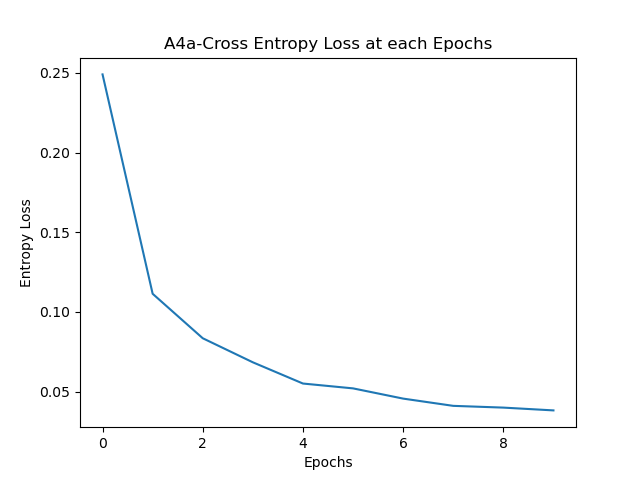
\includegraphics[width=12cm]{A4Mnist/A4(a)-NN-mnist.png}
        \end{center}
        The code is in \hyperref[A.4.code]{A.4.code}
        \\
        The score on the test set is $0.9704$. (Portion of labels it got right)
    \subsection*{A.4.b} 
        \begin{center}
            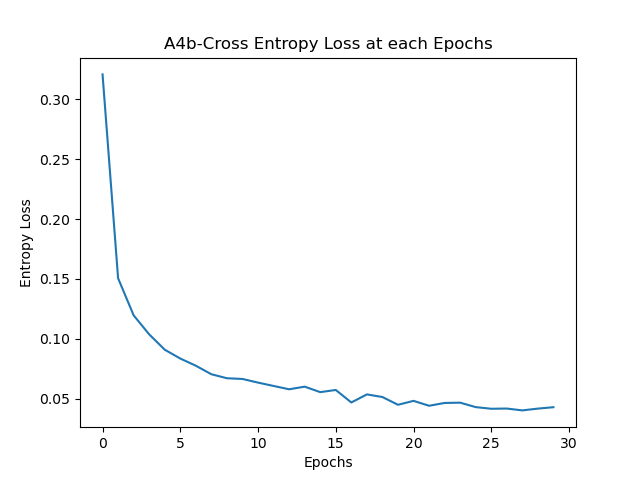
\includegraphics[width=12cm]{A4Mnist/A4(b)-NN-mnist.png}
        \end{center}
        The code is in \hyperref[A.4.code]{A.4.code}
        \\
        The score on the test set is $0.9661$. (Portion of labels it got right)
    \subsection*{A.4.code}\label{A.4.code}
        Here is my implemention of everything in this problem in one file: 
        \\
        File name: ``neural\_net\_mnist.py''
        \begin{lstlisting}
    # This is a code written foor CSE 546 HW3 A4, in spring 2021
    # We are using neural net to distinguish the digits 2, 7 in the MNIST dataset.
    # Author: Hongda Li
    # Don't copy my code it has my style in it.

    import torch
    import torch.nn as nn
    import torch.nn.functional as F
    import torch.optim as optim
    import torchvision.datasets as datasets
    from torchvision import transforms
    from tqdm import tqdm
    from math import sqrt
    from collections import Iterable
    import matplotlib.pyplot as plt

    tensor = torch.tensor
    zeros = torch.zeros
    rand = torch.rand

    MNIST_TRAIN = datasets.MNIST(root="./data",
                                train=True,
                                download=True,
                                transform=transforms.ToTensor())
    # MNIST_TRAIN = torch.utils.data.Subset(MNIST_TRAIN, range(1000))
    MNIST_TEST = datasets.MNIST(root="./data",
                                train=False,
                                download=True,
                                transform=transforms.ToTensor())


    class MyNN:

        def __init__(this, modelParameterMaker:callable):
            """
                Architecture:
                Direct linear stacking of weight and biases. with ReLU.
            :param modelParameterMaker:
                A function that makes the W, weight matrices and the weight vector
                b in the neural network.
            """
            this.Weights, this.Biases = modelParameterMaker()
            assert isinstance(this.Weights, Iterable)
            assert isinstance(this.Biases, Iterable)

        def feedforward(this, X, y):
            """
                X is a row data matrix.
            :param X:
            :param y:
            :return:
            """
            assert X.ndim == 2
            assert X.shape[0] == y.shape[0] or X.shape[1] == y.shape[0]
            a = X  # output of the first layer
            for W, b in list(zip(this.Weights, this.Biases))[:-1]:
                a = F.relu(a@W + b)
            # direct out put from last layer into the loss function.
            a = a @ this.Weights[-1] + this.Biases[-1]
            return F.cross_entropy(a, y)

        def predict(this, X):
            a = X  # output of the first layer
            for W, b in list(zip(this.Weights, this.Biases))[:-1]:
                a = F.relu(a @ W + b)
            a = a @ this.Weights[-1] + this.Biases[-1]
            Probability = F.softmax(a, dim=1)
            return torch.max(Probability, dim=1)[1]


        @property
        def parameters(this):
            # Weights and biases concat together.
            return list(this.Weights) + list(this.Biases)

        @staticmethod
        def A4a():
            """
                Get the parameters ready for A4a.
            :param gpu:
                Whether to use the GPU on the tensor.
            :return:
                2 iterables of the weights and biases.
            """
            W0 = zeros(28 ** 2, 64, requires_grad=True)
            alpha = 1/sqrt(W0.shape[1])
            W0.data += 2*alpha* rand(W0.shape) - alpha
            W1 = zeros(64, 10, requires_grad=True)
            alpha = 1 / sqrt(W1.shape[1])
            W1.data += 2*alpha*rand(W1.shape) - alpha
            b0 = zeros(1,64, requires_grad=True)
            b1 = zeros(1,10, requires_grad=True)
            return [W0, W1], [b0, b1]

        @staticmethod
        def A4b():
            W0 = zeros(28 ** 2, 32, requires_grad=True)
            alpha = 1 / sqrt(W0.shape[1])
            W0.data += 2 * alpha * rand(W0.shape) - alpha

            W1 = zeros(32, 32, requires_grad=True)
            alpha = 1 / sqrt(W1.shape[1])
            W1.data += 2 * alpha * rand(W1.shape) - alpha

            W2 = zeros(32, 10, requires_grad=True)
            alpha = 1 / sqrt(W2.shape[1])
            W2.data += 2 * alpha * rand(W2.shape) - alpha

            b0 = zeros(1, 32, requires_grad=True)
            b1 = zeros(1, 32, requires_grad=True)
            b2 = zeros(1, 10, requires_grad=True)

            return [W0, W1, W2], [b0, b1, b2]


    def main():

        data_loader = torch.utils.data.DataLoader(MNIST_TRAIN,
                                                batch_size=250,
                                                shuffle=True)


        Epochs = 30

        def Accuracy(yhat, y):
            return sum(yhat == y)/yhat.numel()

        def RunMNIST(Model, Optimizer, part):
            EpochLosses = []
            for E in range(Epochs):
                EpochLoss = 0.0
                for X, y, in data_loader:
                    X = X.view(-1, 784)
                    Optimizer.zero_grad()
                    Loss = Model.feedforward(X, y)
                    EpochLoss += Loss.item()/X.shape[0]
                    Loss.backward()
                    Optimizer.step()
                EpochLosses.append(EpochLoss)
                X = torch.stack([D[0].reshape(-1) for D in MNIST_TRAIN], axis=0)
                y = torch.tensor([D[1] for D in MNIST_TRAIN])
                Rate = Accuracy(Model.predict(X), y)
                print(f"Epoch: {E}, Loss: {EpochLoss}")
                print(f"accuracy: {Rate}")
                if Rate > 0.99:
                    print("Process terminated because 99% accuracy reached.")
                    break
            X = torch.stack([D[0].reshape(-1) for D in MNIST_TEST], axis=0)
            y = torch.tensor([D[1] for D in MNIST_TEST])
            TestAccuracy = Accuracy(Model.predict(X), y)
            print(f"Test set accuracy is: {TestAccuracy}")
            plt.plot(EpochLosses)
            plt.title(f"A4{part}-Cross Entropy Loss at each Epochs")
            plt.xlabel("Epochs")
            plt.ylabel("Entropy Loss")
            plt.savefig(f"A4({part})-NN-mnist.png")
            plt.show()
            return TestAccuracy

        Model = MyNN(MyNN.A4a)
        Optimizer = optim.Adam(Model.parameters, lr=0.01)
        Rate = RunMNIST(Model, Optimizer, part="a")
        with open("A4a.txt", "w+") as f:
            f.write(str(Rate))

        Model = MyNN(MyNN.A4b)
        Optimizer = optim.Adam(Model.parameters, lr=0.01)
        Rate = RunMNIST(Model, Optimizer, part="b")
        with open("A4b.txt", "w+") as f:
            f.write(str(Rate))


    if __name__ == "__main__":
        import os
        print(f"cwd:{os.getcwd()} ")
        main()
        \end{lstlisting}
    \subsection*{A.b.c}
        There are 26506 parameters for the deep model and there are 50890 for the shallow model. Usually, it will make sense to have deeper networks, and this is the central hypothesis for many of the existing, famous networks, like the case of the deep residual net. However, it must be clear that, it comes with the risk of overfitting, in addition, the performance will be limited by the width of the hidden layer. This is true because latent variables represent abstract features that network can work with.
        \\
        I would say deeper, larger network is better, and the more parameters the better, if it overfits, we just regularize it. So the second network is better, it manages to achieve accuracy close to the first network all with much less parameters.  
    
\section*{A.5: Using Pretrained Networks and Transfer Learning}
    \textbf{NOTE}: This HW is done with collaborations with another students: Zihao Zhou. 
        \\
        The type of collaboration is: I view his code, and I extract out some of of his stuff in his code that I don't have and made it my own. The stuff he has and I don't are: 
        \begin{enumerate}
            \item[1.] No grad block.
            \item[2.] Data Proprocessing.
            \item[3.] A set of hyperparameters that I can just copy and know it will work.  
            \item[4.] Freeze state\_dict of the model and recover it. 
            \item[5.] The whole idea of storing the best model during training.  
        \end{enumerate}
        \textbf{NOTE}: Version 1.0.1, later version will keep comping, once they are completed. 
        \\
        \textbf{NOTE}: In this version, I divided the loss by the number of batches instead of samples, so they are off by a constant factor. 
        \\
        \textbf{NOTE}: There will be some difference between the code I uploaded into gradescope, and I had several versions on my own google collab, \href{https://colab.research.google.com/drive/1cCKCyvZBUQsXtfZfqKFic64mZy4l99be?usp=sharing}{link}. Last modified: May 21st. The code presented below is one of the instances, the code copied and uploaded to gradescope is code underdevelopment. 
    \subsubsection*{A.5.code}
        \begin{lstlisting}
# This is for CSE SPRING 2021 hw3, A5
# Name: Hongda Li, collaborated with Zihao Zhou

import torch
import torchvision
datasets = torchvision.datasets
transforms = torchvision.transforms
F = torch.nn.functional
nn = torch.nn
optim = torch.optim

import matplotlib.pyplot as plt
import copy

TRANSFORMS  = {
    'train': transforms.Compose([
        transforms.RandomResizedCrop(224),
        transforms.RandomHorizontalFlip(),
        transforms.ToTensor(),
        transforms.Normalize([0.485, 0.456, 0.406], [0.229, 0.224, 0.225])
    ]),
    'test': transforms.Compose([
        transforms.Resize(256),
        transforms.CenterCrop(224),
        transforms.ToTensor(),
        transforms.Normalize([0.485, 0.456, 0.406], [0.229, 0.224, 0.225])
    ]),
}

DEVICE = torch.device("cuda:0" if torch.cuda.is_available() else "cpu")
# DEVICE = "cpu"
CIFAR_TRAIN = datasets.CIFAR10(root="./data",
                                train=True,
                                download=True,
                                transform=TRANSFORMS["train"])
CIFAR_TEST = datasets.CIFAR10(root="./data",
                                train=True,
                                download=True,
                                transform=TRANSFORMS["test"])
CIFAR_TRAIN, CIFAR_VAL = \
        torch.utils.data.random_split(CIFAR_TRAIN, [45000, 50000 - 45000])
# CIFAR_TRAIN, CIFAR_VAL = torch.utils.data.Subset(CIFAR_TRAIN, range(0, 5000, 3)),\
#                          torch.utils.data.Subset(CIFAR_TRAIN, range(1, 5000, 3))
CLASSES = \
    ('plane', 'car', 'bird', 'cat', 'deer', 'dog', 'frog', 'horse', 'ship', 'truck')


class MyCifar:

    def __init__(this, finetune=False):
        Model = torchvision.models.alexnet(pretrained=True)
        if not finetune:
            for Param in Model.parameters():
                Param.require_grad = False
        Model.classifier[-1] = nn.Linear(4096, 10)
        Model.to(DEVICE)
        this.Model = Model
        this.FineTune = finetune

    def __call__(this, *args, **kwargs):
        return this.Model(*args, **kwargs)

    def FeedForward(this, X, y):
        X, y = X.to(DEVICE), y.to(DEVICE)
        return F.cross_entropy(this(X), y)

    def predict(this, X):
        X = X.to(DEVICE)
        return torch.argmax(this(X), axis=1)

    @property
    def Parameters(this):
        if this.FineTune:
            return this.Model.parameters()
        return this.Model.classifier[-1].parameters()


def Run(finetune:bool, batchsize:int, epochs:int):
    Model = MyCifar(finetune=finetune)
    BatchSize = batchsize
    TrainSet = torch.utils.data.DataLoader(CIFAR_TRAIN,
                                            batch_size=BatchSize)
    TrainTotal = len(TrainSet)*BatchSize
    ValSet = torch.utils.data.DataLoader(CIFAR_VAL,
                                            batch_size=BatchSize)
    TestSet = torch.utils.data.DataLoader(CIFAR_TEST, batch_size=BatchSize)
    ValTotal = len(ValSet)*BatchSize
    Optimizer = optim.RMSprop(Model.Parameters, lr=0.0001)
    Epochs = epochs
    TrainLosses, ValLosses, TrainAccuracy, ValAccuracy = [], [], [], []
    BestModel, BestAccuracy = None, 0
    for II in range(Epochs):
        AvgLoss = Correct = 0
        for X, y in TrainSet:
            Optimizer.zero_grad()
            Loss = Model.FeedForward(X, y)
            Loss.backward()
            Optimizer.step()
            with torch.no_grad():
                AvgLoss += float(Model.FeedForward(X, y)) / len(TrainSet)
                Correct += float(torch.sum(Model.predict(X).to("cpu") == y))/TrainTotal
        TrainLosses.append(AvgLoss)
        TrainAccuracy.append(Correct)
        print(f"Epoch: {II}, Train Loss: {AvgLoss}, Train Acc: {TrainAccuracy[-1]}", end="; ")
        Correct = AvgLoss = 0
        for X, y in ValSet:
            with torch.no_grad():
                Loss = Model.FeedForward(X, y)
                Correct += float(torch.sum(Model.predict(X).to("cpu") == y))/ValTotal
            AvgLoss += float(Loss)/len(ValSet)
        ValAccuracy.append(Correct)
        ValLosses.append(AvgLoss)
        print(f"Val Loss: {AvgLoss}, Val Acc: {ValAccuracy[-1]}")
        if ValAccuracy[-1] > BestAccuracy:
            BestAccuracy = ValAccuracy[-1]
            BestModel = copy.deepcopy(Model.Model.state_dict())

    # Plot train, val losses
    plt.plot(TrainLosses)
    plt.plot(ValLosses)
    plt.legend(["Train Loss", "Val Loss"])
    plt.title(f"Train and Validation Loss, finetune: {finetune}")
    plt.xlabel("Epoch")
    plt.savefig(f"A5a-train-val-loss-{finetune}.png")
    plt.show()

    # Plot train val acc
    plt.plot(TrainAccuracy)
    plt.plot(ValAccuracy)
    plt.legend(["Train Acc", "Val Acc"])
    plt.title(f"Train and Validation Accuracy, finetune: {finetune}")
    plt.xlabel("Epoch")
    plt.savefig(f"A5a-train-val-acc-{finetune}.png")
    plt.show()

    # Test Accuracy
    TestAcc = 0
    Model = MyCifar()
    Model.Model.load_state_dict(BestModel)
    Model.Model.eval()
    for X, y in TestSet:
        with torch.no_grad():
            TestAcc += torch.sum(Model.predict(X).to("cpu") == y)/len(CIFAR_TEST)
    print(f"TestAcc: {TestAcc}")
    with open("a5-test-acc.txt", "w+") as f:
        f.write(str(TestAcc))
    return Model


def main():
    Run(False, 100, epochs=20)
    Run(True, 100, epochs=20)

if __name__ == "__main__":
    import os
    print(f"current dir:{os.curdir}")
    print(f"cwd: {os.getcwd()}")
    Model = main()
        \end{lstlisting}
    
    \subsubsection*{A.5.a}
        The final test error is: $0.8136000633239746$. 
        \begin{center}
            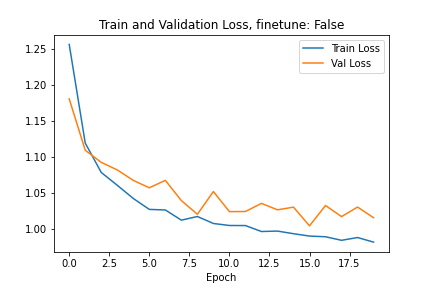
\includegraphics[width=12cm]{a5plots/A5a-train-val-loss-False1.png}
            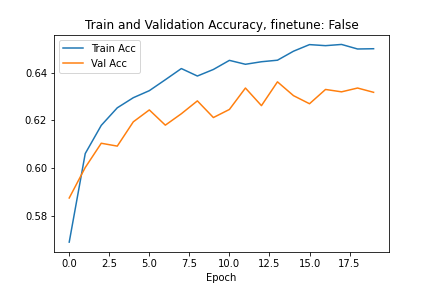
\includegraphics[width=12cm]{a5plots/A5a-train-val-acc-False1.png}
        \end{center}
        Hyper Parameters: 
        \begin{enumerate}
            \item[1.] BatchSize = 100
            \item[2.] Learning Rate = 0.0001 
        \end{enumerate}
        Why test accuracy so high? Data Pre-processing and data augmentation? 
    
    \subsubsection*{A.5.b}
        The final test error is: $0.9650202989578247$. 
        \begin{center}
            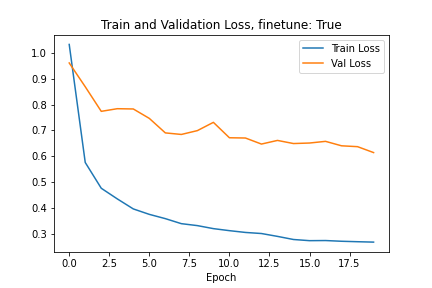
\includegraphics[width=12cm]{a5plots/A5a-train-val-loss-True1.png}
            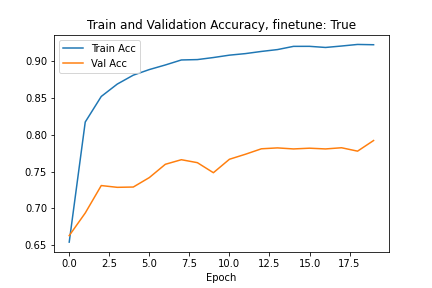
\includegraphics[width=12cm]{a5plots/A5a-train-val-acc-True1.png}
        \end{center}
        Why test accuracy so high? Data Pre-processing and data augmentation? 
        \begin{enumerate}
            \item[1.] BatchSize = 100
            \item[2.] Learning Rate = 0.0001 
        \end{enumerate}

\section*{A.6: Image Classification on CIFAR-10}
    \textbf{Notes}: 
        I am unable to complete this part of the HW because I am not willingly to spend time on this HW with expense on my other classes and assignments, I am not using the late days because it comes with an opportunity cost. 
        \\
        Here is a list of things I did for this part: 
        \begin{enumerate}
            \item[$\bullet$] Usage of SHGO algorithm for optimizing the model accuracy by tunning the hyperparameters. SHGO is provided by scipy for global constrained blackbox optimization. 
            \item[$\bullet$] A whole automated process for hyper tuning and model selection is deployed. 
            \item[$\bullet$] Top 9 models with maximum cross validations accuracy are received and visualized. 
            \item[$\bullet$] I automated the whole process of model selections from hypertuning, and the computational results are saved.  
            \item[$\bullet$] \textbf{Batchsize is not involved as a hyperparameter} for (b), (c) because there is this weird relation where, higher learning rate and larger batchsizes gives similar accuracy as smaller training rate and smaller batchsizes, therefore, I fixed the batch size and only focuses on learning rate. These 2 quantities are interacting with each other. Interesting. Therefore I fixed the batchsize to be 100 for all model, for all training in (b), (c) to save some time. 
            \item[$\bullet$] The accuracy of the first epochs is measured after the gradient descend step. This is the case for all epochs. That is why all the accuracy started somehwere above 
        \end{enumerate}
        This is my code implementation that produces everything: 
        \\
        File name: ``A6.py''
        \begin{lstlisting}[language=python]
# name: Hongda Li
# This is for A6 HW3 CSE 546 SPRING 2021
# Don't copy my code it has my style in it.


import torch
import torchvision
datasets = torchvision.datasets
transforms = torchvision.transforms
F = torch.nn.functional
nn = torch.nn
optim = torch.optim
sqrt = torch.sqrt
from tqdm import tqdm

from scipy.optimize import shgo
import matplotlib.pyplot as plt
import copy

TRANSFORMS = {
    'train': transforms.Compose([
        transforms.ToTensor(),
    ]),
    'val': transforms.Compose([
        transforms.ToTensor(),
    ]),
}

DEVICE = torch.device("cuda:0" if torch.cuda.is_available() else "cpu")

#DEVICE = "cpu"
CIFAR_TRAIN = datasets.CIFAR10(root="./data",
                                train=True,
                                download=True,
                                transform=TRANSFORMS["val"])
CIFAR_TEST = datasets.CIFAR10(root="./data",
                                train=True,
                                download=True,
                                transform=TRANSFORMS["val"])
CIFAR_TRAIN, CIFAR_VAL = \
        torch.utils.data.random_split(CIFAR_TRAIN,
                                    [45000, 50000 - 45000])
# CIFAR_TRAIN, CIFAR_VAL = torch.utils.data.Subset(CIFAR_TRAIN,
#                                                  range(0, 10000)),\
#                          torch.utils.data.Subset(CIFAR_TRAIN,
#                                                  range(10000, 10000 + 1000))
CLASSES = \
    ('plane', 'car', 'bird', 'cat', 'deer', 'dog', 'frog', 'horse', 'ship', 'truck')


def BatchThisModel(theModel, theDataLoader, optimizer=None, dataTransform:callable=None):
    """
        Performs one epochs of training or inference, depending on whether
        optimizer is None or not.
    :param theModel:
    :param theDataLoader:
    :param optimizer:
    :return:
    """
    theModel.to(DEVICE)
    AvgLoss = 0
    AvgAccuracy = 0
    for X, y in theDataLoader:
        if dataTransform:
            X = dataTransform(X)
        X, y= X.to(DEVICE), y.to(DEVICE)
        if optimizer is not None: # GD
            optimizer.zero_grad()
            Loss = theModel.FeedForward(X, y)
            AvgLoss += Loss.item()
            Loss.backward()
            optimizer.step()

        else: # Inference
            with torch.no_grad():
                Loss = theModel.FeedForward(X, y)
                AvgLoss += Loss.item()
        with torch.no_grad():
            AvgAccuracy +=\
                float(torch.sum(theModel.predict(X) == y)/(len(theDataLoader)*len(y)))
    return AvgAccuracy

def GetTrainValDataLoader(bs):
    TrainSet = torch.utils.data.DataLoader(CIFAR_TRAIN,
                                            batch_size=bs)
    ValSet = torch.utils.data.DataLoader(CIFAR_VAL,
                                            batch_size=bs)
    return TrainSet, ValSet

def GetTS():
    import time
    Ts = time.strftime('%H-%M-%S-%b-%d-%Y')
    return Ts



class BestModelRegister:
    """
    Pass to the trainer and stores all the losses and data from the training process.
    """
    def __init__(this):
        this.BestModel = None
        this.ModelType = None
        # Hyper parameters maps to Epochs Acc
        this.HyperParameterAccList = {}
        # Best Acc maps to best Params tuple
        this.BestAccToParams = {}
        # Absolute Best ACC from whatever agorithm run the hypertune.
        this.BestAcc = 0

    def save(this):
        import time
        from pathlib import Path
        Path("./a6bestmodel").mkdir(parents=True, exist_ok=True)
        torch.save(this.BestModel.state_dict(), f"./a6bestmodel/{time.strftime('%H-%M-%S-%b-%d-%Y')}")

    def Top9AccList(this):
        """
            Get the hyper params with top 10 accuracy.
        :return:
        """
        List = list(this.BestAccToParams.keys())
        List.sort(reverse=True)
        List = List[:min(9, len(List))]
        Result = {}
        for K in List:
            Result[K] = this.HyperParameterAccList[this.BestAccToParams[K]]
        return Result

    def ProducePlotPrintResult(this):
        from pathlib import Path
        Path("./a6bestmodel").mkdir(parents=True, exist_ok=True)
        import time
        Ts = time.strftime('%H-%M-%S-%b-%d-%Y')

        ModelTypeMap = {1: "Logistic", 2: "Single Hidden", 3:"CNN"}
        TheLegends = [1, 2, 3, 4, 5, 6, 7, 8, 9]
        TopList = this.Top9AccList()
        # Plot the training acc
        for _, V in TopList.items():
            plt.plot(V[0])
        plt.xlabel("Epochs")
        plt.ylabel("Their Train acuracy")
        plt.title(f"Model: {ModelTypeMap[this.ModelType]} Top 9 ranked by peak val acc")
        plt.legend([f"top {R}" for R in TheLegends])
        plt.savefig(f"./a6bestmodel/{Ts}-{ModelTypeMap[this.ModelType]}-train-acc.png")
        plt.show()
        # Plot the validation acc
        for _, V in TopList.items():
            plt.plot(V[1])
        plt.xlabel("Epochs")
        plt.ylabel("Their Val acuracy")
        plt.title(f"Model: {ModelTypeMap[this.ModelType]} Top 9 ranked by peak val acc")
        plt.legend([f"top {R}" for R in TheLegends])
        plt.savefig(f"./a6bestmodel/{Ts}-{ModelTypeMap[this.ModelType]}-val-acc.png")
        plt.show()
        # Plot the top 1 model found:
        plt.plot(TopList[max(TopList.keys())][0])
        plt.plot(TopList[max(TopList.keys())][1])
        plt.legend(["train", "val"])
        plt.xlabel("epochs")
        plt.ylabel("acc")
        plt.title("Best model train val acc")
        plt.savefig(f"./a6bestmodel/{Ts}-{ModelTypeMap[this.ModelType]}-best-acc.png")
        plt.show()
        # write the results


        with open(f"./a6bestmodel/top9A6-{Ts}" +
                    f"-{ModelTypeMap[this.ModelType]}.txt", "w+") as f:
            if this.ModelType == 1:

                f.write(f"max_val_acc, BatchSize, Learning_Rate\n")
                for K, _ in TopList.items():
                    Params = this.BestAccToParams[K]
                    f.write(f"{K}, {Params[0]}, {Params[1]}\n")
            elif this.ModelType == 2:
                f.write(f"max_val_acc, BatchSize, Learning_Rate, Hidden_Layer_width\n")
                for K, _ in TopList.items():
                    Params = this.BestAccToParams[K]
                    f.write(f"{K}, {Params[0]}, {Params[1]}, {Params[2]}\n")
            elif this.ModelType == 3:
                f.write(f"max_val_acc, BatchSize, Learning_Rate, Num_Channels, Conv_Kernel, MaxPool_Kernel\n")
                for K, _ in TopList.items():
                    Params = this.BestAccToParams[K]
                    f.write(f"{K}, {Params[0]}, {Params[1]}, {Params[2]}, {Params[3]}, {Params[4]}\n")
            else:
                assert False, "Unrecognized type, or not yet implemented"




class ModelA(nn.Module):
    def __init__(this):
        super().__init__()
        this.Linear = nn.Linear(3*32**2, 10)

    def FeedForward(this, X, y):
        yhat = this(X)
        return F.cross_entropy(yhat, y)

    def forward(this, X):
        x = this.Linear(X)
        return x

    def predict(this, X):
        return torch.argmax(this(X), axis=1)

    @staticmethod
    def GetHyperTuneFunc(Epochs, verbose, modelRegister):
        modelRegister.ModelType = 1
        def flatten(x):
            return x.view(x.shape[0], -1)
        def HyperTuneFunc(x, mem={}):
            """
            This function is passed to SHGO for optimization.
            :param x:
            :param mem:
            :return:
            """
            BatchSize, Lr = int(x[0]), x[1]
            if (BatchSize, Lr) in mem:
                return mem[BatchSize, Lr]
            Model = ModelA()
            if verbose: print(f"ModelA, Hypertune, Bs: {BatchSize}, lr: {Lr}")
            Optimizer = optim.Adam(Model.parameters(), lr=Lr)
            T, V = GetTrainValDataLoader(BatchSize)
            BestAcc = -float("inf")
            TrainAcc, ValAcc = [], []
            for II in tqdm(range(Epochs)):
                Acc = BatchThisModel(Model, T, optimizer=Optimizer, dataTransform=flatten)
                TrainAcc.append(Acc)
                Acc = BatchThisModel(Model, V, dataTransform=flatten)
                ValAcc.append(Acc)
                if Acc > BestAcc:
                    BestAcc = Acc
            modelRegister.HyperParameterAccList[BatchSize, Lr] = (TrainAcc, ValAcc)
            modelRegister.BestAccToParams[BestAcc] = (BatchSize, Lr)
            if Acc > modelRegister.BestAcc:
                modelRegister.BestAcc = Acc
                modelRegister.BestModel = Model
                if verbose: print(f"Best Acc Update: {Acc}")
            mem[BatchSize, Lr] = 1 - Acc # Memeorization.
            return 1 - Acc
        return HyperTuneFunc


class ModelB(nn.Module):
    def __init__(this, hiddenWidth):
        super().__init__()
        this.L1 = nn.Linear(3*32**2, hiddenWidth)

    def FeedForward(this, X, y):
        return F.cross_entropy(this(X), y)

    def forward(this, X):
        x = this.L1(X)
        x = F.relu(x)
        return x

    def predict(this, X):
        return torch.argmax(this(X), axis=1)

    @staticmethod
    def GetHyperTuneFunc(Epochs, verbose, modelRegister):
        modelRegister.ModelType = 2
        def flatten(x):
            return x.view(x.shape[0], -1)
        def HyperTuneFunc(x, mem={}):
            """
            This function is passed to SHGO for optimization.
            :param x:
            :param mem:
            :return:
            """
            BatchSize, Lr, HiddenLayerWidth= int(x[0]), x[1], int(x[2])
            if (BatchSize, Lr, HiddenLayerWidth) in mem:
                return mem[BatchSize, Lr, HiddenLayerWidth]
            Model = ModelB(HiddenLayerWidth)
            if verbose: print(f"ModelB, Hypertune, Bs: {BatchSize}, lr: {Lr}, HLW: {HiddenLayerWidth}")
            Optimizer = optim.Adam(Model.parameters(), lr=Lr)
            T, V = GetTrainValDataLoader(BatchSize)
            BestAcc = -float("inf")
            TrainAcc, ValAcc = [], []
            for II in tqdm(range(Epochs)):
                Acc = BatchThisModel(Model, T, optimizer=Optimizer, dataTransform=flatten)
                TrainAcc.append(Acc)
                Acc = BatchThisModel(Model, V, dataTransform=flatten)
                ValAcc.append(Acc)
                if Acc > BestAcc:
                    BestAcc = Acc
            modelRegister.HyperParameterAccList[BatchSize, Lr, HiddenLayerWidth] = (TrainAcc, ValAcc)
            modelRegister.BestAccToParams[BestAcc] = (BatchSize, Lr, HiddenLayerWidth)
            if Acc > modelRegister.BestAcc:
                modelRegister.BestAcc = Acc
                modelRegister.BestModel = Model
                if verbose: print(f"Best Acc Update: {Acc}")
            mem[BatchSize, Lr, HiddenLayerWidth] = 1 - Acc  # Memeorization.
            return 1 - Acc

        return HyperTuneFunc


class ModelC(torch.nn.Module):
    def __init__(this, c, k1, k2):
        """

        :param c:
            Chennel for conv2d
        :param k1:
            Kernel for conv2d
        :param k2:
            Kernel for max pool
        """
        super().__init__()
        this.Con = nn.Conv2d(3, c, k1)
        this.Mp = nn.MaxPool2d(k2, k2)
        Width = int((32 - k1 + 1)/k2)
        this.L1 = nn.Linear(c*Width**2, 10)

    def FeedForward(this, X, y):
        return F.cross_entropy(this(X), y)

    def forward(this, X):
        x = this.Con(X)
        x = F.relu(x)
        x = this.Mp(x)
        x = torch.flatten(x, 1)
        return this.L1(x)

    def predict(this, X):
        return torch.argmax(this(X), axis=1)


    @staticmethod
    def GetHyperTuneFunc(Epochs, verbose, modelRegister):
        modelRegister.ModelType = 3
        def HyperTuneFunc(x, mem={}):
            """
            This function is passed to SHGO for optimization.
            :param x:
            :param mem:
            :return:
            """
            BatchSize, Lr, Channels, Kernel1, Kernel2 = \
                int(x[0]), x[1], int(x[2]), int(x[3]), int(x[4])
            if (BatchSize, Lr, Channels, Kernel1, Kernel2) in mem:
                return mem[BatchSize, Lr, Channels, Kernel1, Kernel2]
            Model = ModelC(Channels, Kernel1, Kernel2)
            if verbose: print(f"ModelC, Bs: {BatchSize}, lr: {Lr}," +
                                f" Channels: {Channels}, K1: {Kernel1}, K2: {Kernel2}")
            Optimizer = optim.Adam(Model.parameters(), lr=Lr)
            T, V = GetTrainValDataLoader(BatchSize)
            BestAcc = -float("inf")
            TrainAcc, ValAcc = [], []
            for II in tqdm(range(Epochs)):
                Acc = BatchThisModel(Model, T, optimizer=Optimizer)
                TrainAcc.append(Acc)
                Acc = BatchThisModel(Model, V)
                ValAcc.append(Acc)
                if Acc > BestAcc:
                    BestAcc = Acc
            modelRegister.HyperParameterAccList[BatchSize, Lr, Channels, Kernel1, Kernel2] \
                = (TrainAcc, ValAcc)
            modelRegister.BestAccToParams[BestAcc] = (BatchSize, Lr, Channels, Kernel1, Kernel2)
            if Acc > modelRegister.BestAcc:
                modelRegister.BestAcc = Acc
                modelRegister.BestModel = Model
                if verbose: print(f"Best Acc Update: {Acc}")
            mem[BatchSize, Lr, Channels, Kernel1, Kernel2] = 1 - Acc  # Memeorization.
            return 1 - Acc

        return HyperTuneFunc


def main():
    def TuneModel1():
        ModelRegister = BestModelRegister()
        TheFunc = ModelA.GetHyperTuneFunc(20, True, ModelRegister)
        result = shgo(TheFunc,
                [(10, 500), (5e-6, 0.01)],
                options={"maxev":50, "ftol": 1e-2, "maxfev": 10})
        print(result)
        print(ModelRegister.Top9AccList())
        ModelRegister.ProducePlotPrintResult()
        TestSet = torch.utils.data.DataLoader(CIFAR_VAL,
                                            batch_size=2000)
        Acc = BatchThisModel(ModelRegister.BestModel,
                                TestSet,
                                dataTransform=lambda x: x.view(x.shape[0], -1))
        with open(f"./a6bestmodel/{GetTS()}-best-model-logistic-test.txt", "w+") as f:
            f.write(str(Acc))


    def TuneModel2():
        ModelRegister = BestModelRegister()
        TheFunc = ModelB.GetHyperTuneFunc(20, True, ModelRegister)
        result = shgo(TheFunc,
                        [(100, 100), (1e-6, 0.01), (20, 3000)],
                        options={"maxev": 20, "ftol": 1e-2, "maxfev": 10})
        print(result)
        print(ModelRegister.Top9AccList())
        ModelRegister.ProducePlotPrintResult()
        TestSet = torch.utils.data.DataLoader(CIFAR_VAL,
                                                batch_size=2000)
        Acc = BatchThisModel(ModelRegister.BestModel, TestSet,
                                dataTransform=lambda x: x.view(x.shape[0], -1))
        with open(f"./a6bestmodel/{GetTS()}-best-model-hidden-test.txt", "w+") as f:
            f.write(str(Acc))

    def TuneModel3():
        ModelRegister = BestModelRegister()
        TheFunc = ModelC.GetHyperTuneFunc(20, True, ModelRegister)
        result = shgo(TheFunc,
                        [(100, 100), (1e-6, 0.01), (10, 200), (2, 5), (2, 4)],
                        options={"maxev": 20, "ftol": 1e-2, "maxfev": 10})
        print(result)
        print(ModelRegister.Top9AccList())
        ModelRegister.ProducePlotPrintResult()
        TestSet = torch.utils.data.DataLoader(CIFAR_VAL,
                                                batch_size=2000)
        Acc = BatchThisModel(ModelRegister.BestModel, TestSet)
        with open(f"./a6bestmodel/{GetTS()}-best-model-cnn-test.txt", "w+") as f:
            f.write(str(Acc))
        pass
    # TuneModel2()
    TuneModel1()
    # TuneModel3()

if __name__ == "__main__":
    import os
    print(f"curdir: {os.curdir} ")
    print(f"cwd: {os.getcwd()}")
    print(f"Pytorch device: {DEVICE}")
    main()            
        \end{lstlisting}
    \subsubsection*{A.6.a}
        This is some of the top ranking parameters for the logistic model: 
        \begin{lstlisting}
max_val_acc,       BatchSize, Learning_Rate
0.41112577077001333, 132,       0.0025037649011611937
0.4107545465230942,  132,       0.00250375
0.4018739815801382,  377,       0.0025037649011611937
0.39831049367785454, 377,       0.00250375
0.39319999516010284, 500,       0.01
0.38413627818226814, 132,       0.00750125
0.3807273795828223,  255,       0.01
0.3755999828426866,  10,        5e-06
0.37519998475909233, 500,       0.0050025
        \end{lstlisting}
        And this is the performance of these model for all epochs, they are ranked by maximal achieved validations acurracy. 
        \\
        \begin{center}
            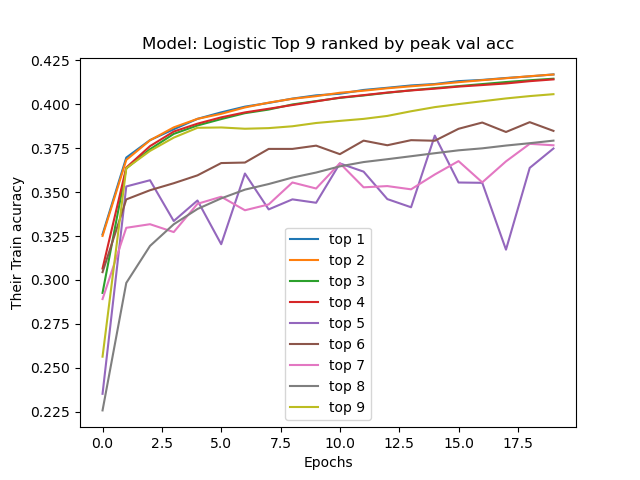
\includegraphics[width=12cm]{a6plots/20-37-33-May-22-2021-Logistic-train-acc.png}
            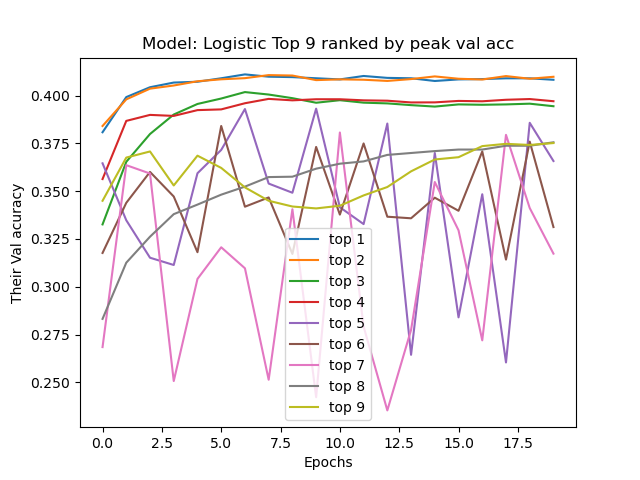
\includegraphics[width=12cm]{a6plots/20-37-33-May-22-2021-Logistic-val-acc.png}
        \end{center}
        And this is the best model's performance on the training set over all training and validtion accuracy. 
        \begin{center}
            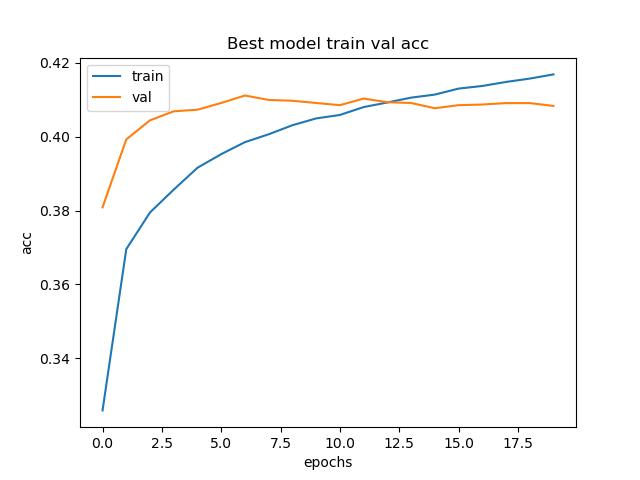
\includegraphics[]{a6plots/20-37-33-May-22-2021-Logistic-best-acc.png}
        \end{center}
        The accuracy of the best model on the test set is: $0.41099999845027924$
        \\
        Used optimizer: Adam. 
        \\
        Momentum: Didn't set. 
    \subsubsection*{A.7.b}
        And this is a list of hyperparameters for the top ranking Hidden Layer model: 
        \begin{lstlisting}
max_val_acc,     BatchSize, Learning_Rate,    Hidden_Layer_width
0.3471999899484217,  100, 0.0025007500000000004, 765
0.3235999927856028,  100, 0.002500764901161194,  765
0.32199999084696174, 100, 0.0025007500000000004, 2255
0.3065999918617308,  100, 0.007500250000000001,  765
0.305199992377311,   100, 0.01,                  3000
0.30419999407604337, 100, 0.002500764901161194,  2255
0.2867999942973256,  100, 1e-06,                 20
0.2729999946895987,  100, 0.005000500000000001,  3000
0.26119999354705215, 100, 0.005000500000000001,  1510
        \end{lstlisting}
        And this is their training behaviors for all of these top ranking parameters: 
        \begin{center}
            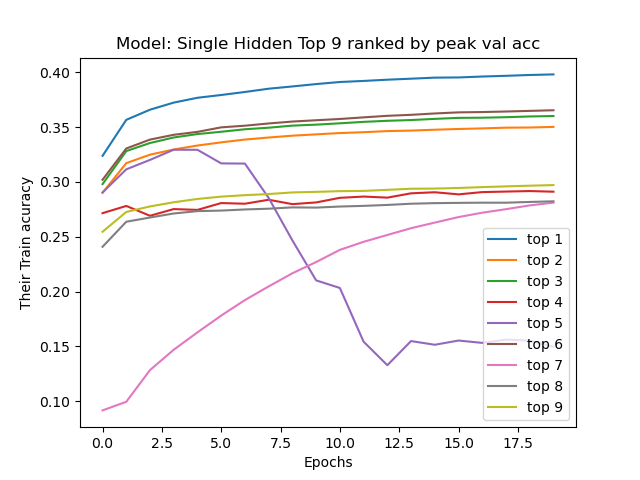
\includegraphics[width=12cm]{a6plots/20-16-57-May-22-2021-Single Hidden-train-acc.png}
            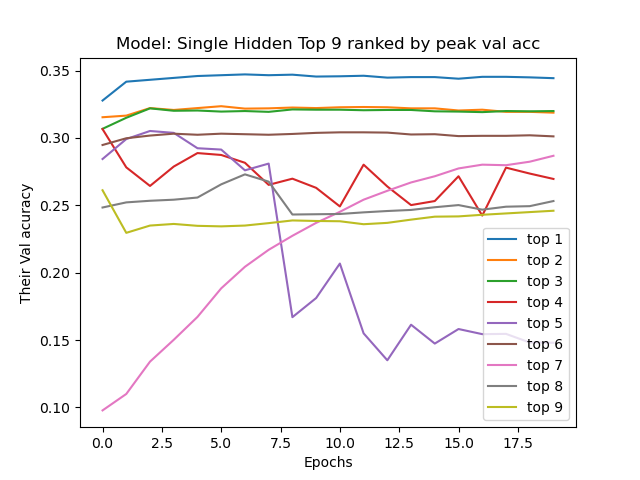
\includegraphics[width=12cm]{a6plots/20-16-57-May-22-2021-Single Hidden-val-acc.png}
        \end{center}
        \begin{center}
            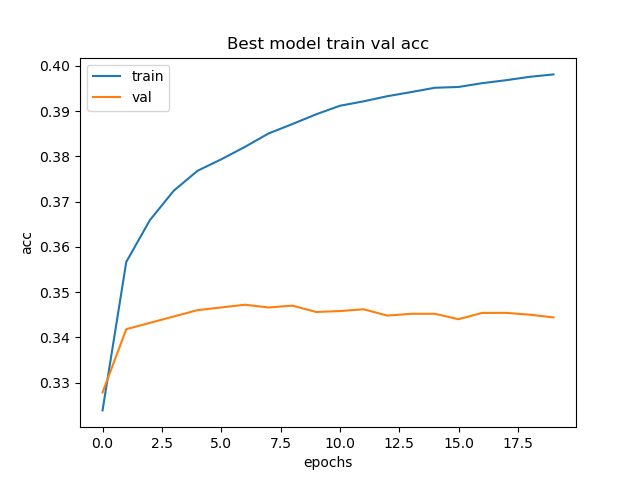
\includegraphics[width=12cm]{a6plots/20-16-57-May-22-2021-Single Hidden-best-acc.png}
        \end{center}
        And the test set accuracy achieved by the best model is: $0.34299998730421066$
        The optimizer is Adam and momentum is not set. 
    \subsection{A.7.c}
        These are some of the models with top ranking validations accuracy, and their parameters are: 
        \begin{lstlisting}
max_val_acc, BatchSize, Learning_Rate, Num_Channels, Conv_Kernel, MaxPool_Kernel
0.6393999857828021,  100, 0.0050005149011611945, 105, 3, 3
0.6305999839678407,  100, 0.005000500000000001,  105, 3, 3
0.6079999813809991,  100, 0.01,                  200, 2, 4
0.5557999834418297,  100, 0.01,                  10,  2, 4
0.5539999827742577,  100, 0.01,                  200, 5, 4
0.5407999884337187,  100, 0.01,                  200, 2, 2
0.5085999895818532,  100, 0.01,                  10,  2, 2
0.5043999869376421,  100, 0.01,                  10,  5, 4
0.48519998881965876, 100, 0.01,                  200, 5, 2
        \end{lstlisting}

        And these are the training behaviors for these best ranking model: 
        \begin{center}
            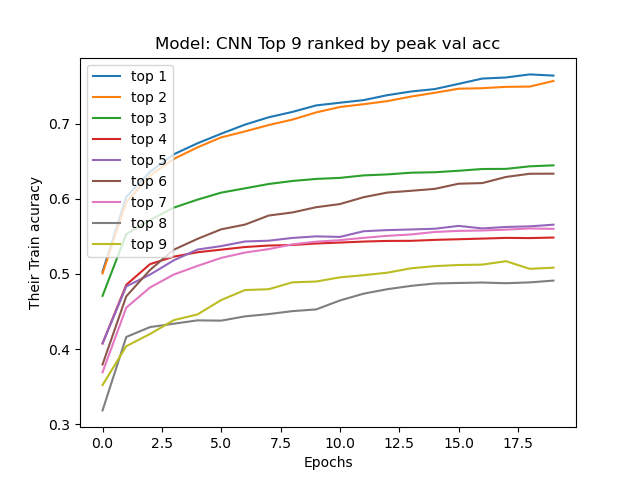
\includegraphics[width=12cm]{a6plots/20-47-34-May-22-2021-CNN-train-acc.png}
            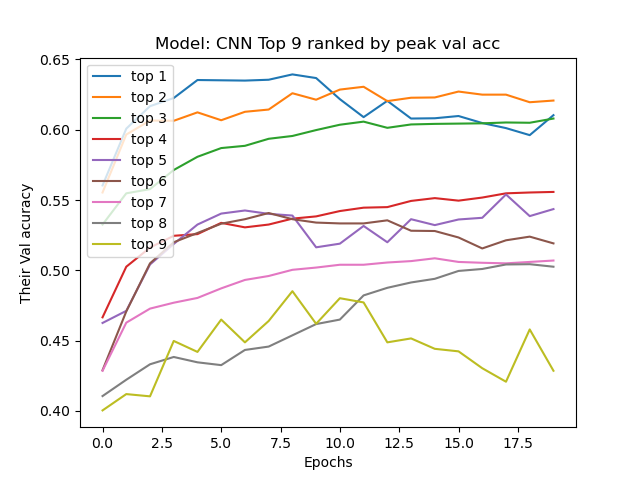
\includegraphics[width=12cm]{a6plots/20-47-34-May-22-2021-CNN-val-acc.png}
        \end{center}
        \begin{center}
            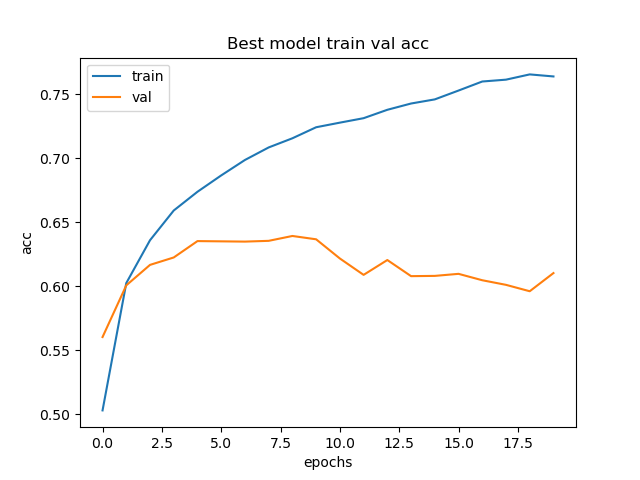
\includegraphics[width=12cm]{a6plots/20-47-34-May-22-2021-CNN-best-acc.png}
        \end{center}
        And the accuracy evaluated on the test set is: $0.6218333095312119$
        \\
        The optimizer is adam, and the momentum is not set. 
    \section*{A.7.c}
        Now, I don't have time to do this HW anymore, if you were excuse me, I need to make quizes because I am a TA, I also need to do c++ programming and fighting with PDEs in 3D using Sturmm Louville's Theory. Convlutional network is only part of life. 
        \\
        I also don't decide to put too much effort for this class at the expense of other class, because there is a diminishing return between the amount of effort and the actualy stuff I learn. 
        \\
        Yeah...
        
\end{document}
